\documentclass[tikz]{standalone}
\usetikzlibrary{arrows, positioning}
\usetikzlibrary {arrows.meta}
\usepackage{xcolor}
\definecolor{allcolor}{RGB}{148,182,233}
\newcommand*{\equal}{=}
\begin{document}
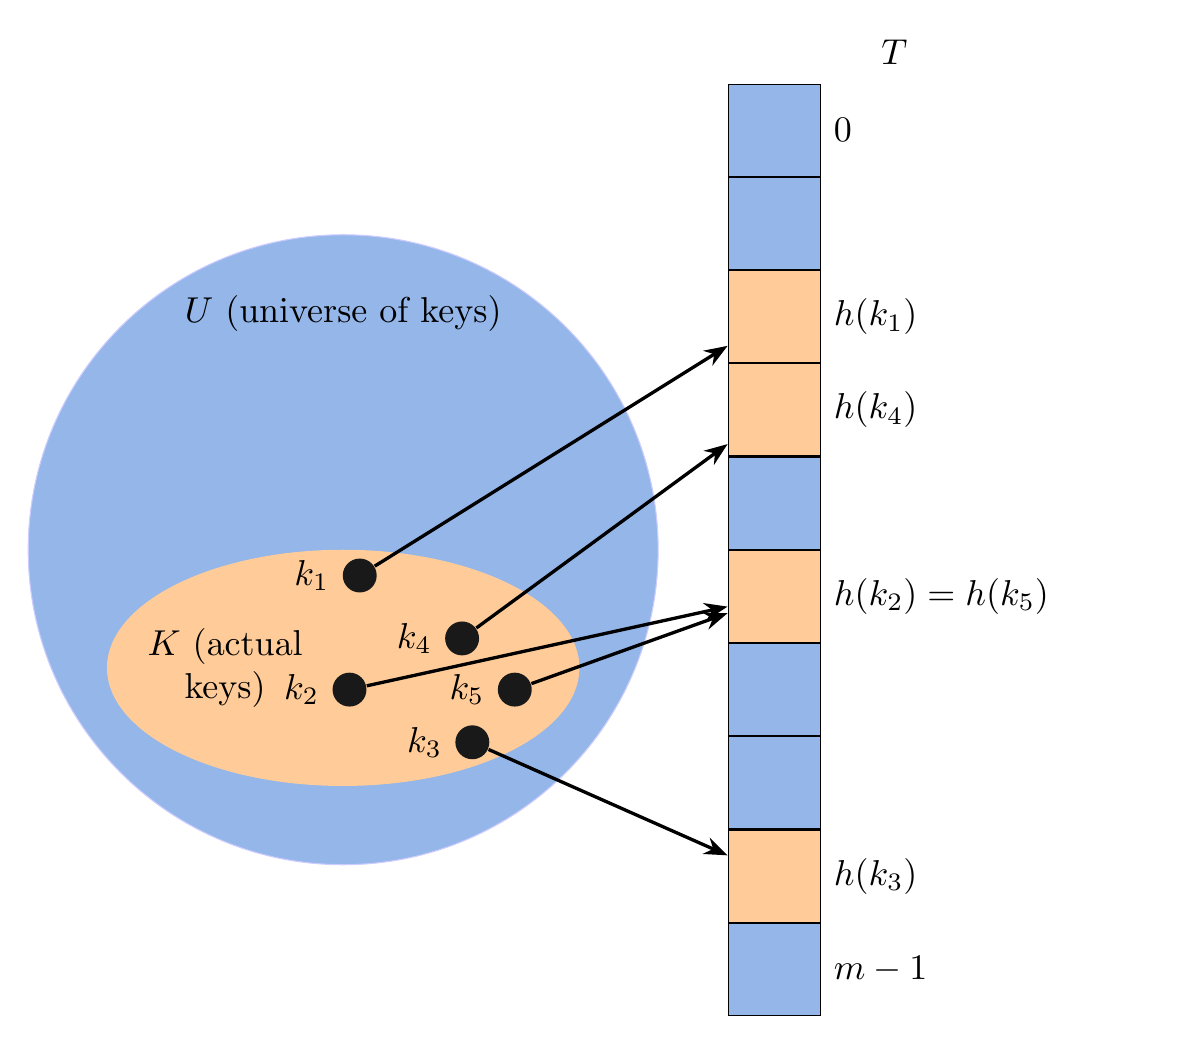
\begin{tikzpicture}[every node/.style={scale=1.3}, dot/.style={minimum size=0.1mm, circle, fill=black!90}, slot/.style={minimum size=0.9cm, rectangle}, noslot/.style={slot, fill=allcolor},
    yesslot/.style={slot, fill=orange!40}, data/.style={minimum size=0.7cm, fill=orange!40}, >=Stealth]
    \tikzstyle{textbf} = [text width=5cm,text centered]

    \filldraw[color=blue!20, fill=allcolor](0,0) circle (4);
    \node[textbf] (universe) at (0, 3) {$U$ (universe of keys)};

    \fill[orange!40] (0, -1.5) ellipse (3 and 1.5);
    \node[textbf, text width=2cm] (keys) at (-1.5, -1.5) {$K$ (actual keys)};

    \node[dot, label=left:$k_1$] [above right=of keys, xshift=-0.7cm, yshift=-0.5cm] (k1){};
    \node[dot, label=left:$k_4$, xshift=1cm, yshift=0.5cm] [below=of k1] (k4){};
    \node[dot, label=left:$k_2$] [below=of k1, xshift=-0.1cm] (k2){};
    \node[dot, label=left:$k_3$] [below=of k4, yshift=0.1cm, xshift=0.1cm] (k3){};
    \node[dot, label=left:$k_5$] [right=of k2, xshift=0.5cm] (k5){};

    \matrix [column sep=1cm,nodes=draw] (table) at (7, 0)
    {
      \node[noslot, label=right:$0$] {}; \\
      \node[noslot] {}; \\
      \node[yesslot, label=right:$h(k_1)$] (s2) {}; \\
      \node[yesslot, label=right:$h(k_4)$] (s3) {}; \\
      \node[noslot] {}; \\
      \node[yesslot, label=right:$h(k_2)\equal h(k_5)$] (s5) {}; \\
      \node[noslot] {}; \\
      \node[noslot] {}; \\
      \node[yesslot, label=right:$h(k_3)$] (s8) {}; \\
      \node[noslot, label=right:$m - 1$] {}; \\
    };

    \node[textbf, above=of table,yshift=-0.8cm]{$T$};
    \draw[->, very thick]  (k1) to (s2);
    \draw[->, very thick]  (k4) to (s3); 
    \draw[->, very thick]  (k2) to (s5);
    \draw[->, very thick] (k3) to (s8);
    \draw[->, very thick] (k5) to (s5);

    
\end{tikzpicture}
\end{document}